\documentclass[14pt,a4paper]{article} %openany
\usepackage[affil-it]{authblk}
\usepackage[english]{babel}
\usepackage{graphicx}
\usepackage{rotating}
\usepackage{amsmath}
\usepackage{adjustbox}
\usepackage{courier}
\usepackage{verbatim}
\usepackage{url}
\usepackage{float}
\usepackage{array}
\usepackage{breakcites}
\usepackage{gensymb}
\usepackage{booktabs,tabularx}
\usepackage{listings}


\renewcommand{\tabularxcolumn}{m}
\renewcommand{\listfigurename}{List of Figures and Tables}


\begin{document}

\begin{titlepage}
    \begin{center}
       % \vspace*{1cm}
        
        \Huge
        \textbf{NPRE 247 CP3}
        
        \vspace{0.5cm}
        \LARGE

        \textbf{Anshuman Chaube}\\
        Due 12/4/17
       
 
                
    \end{center}
\end{titlepage}

%\frontmatter{}
%
 % \tableofcontents
\newpage


\section{Fuel enrichment(weight \% ) in given Serpent input}
For the given atomic concentration of 5 \% for \textsuperscript{235}U, the enrichement was found to be \textbf{4.358 \% w/w}.

\section{Cladding Composition}

\begin{tabular}{c c c c}

\textbf{Z} & \textbf{Element} & \textbf{Mass Fraction} & \textbf{Atom \%} \\
40         & Zr               &  0.9823                &   98.3649         \\
50         & Sn               &  0.0145                &    1.1158         \\
26         & Fe               &  0.0021                &    0.3435         \\
24         & Cr               &  0.0010                &    0.1757         \\
72         & Hf               &  0.0001                &   $5.12x10^{-4}$  \\
\end{tabular}

\section{Optimum fuel to moderator ratio}

The optimum fuel to moderator ratio was found to be \textbf{3.25910}, corresponding to a k (K\_IMP) value of 1.16768 and moderator density 1.11 g/mL.

\section{Plot}

\begin{figure}[H]
\centering
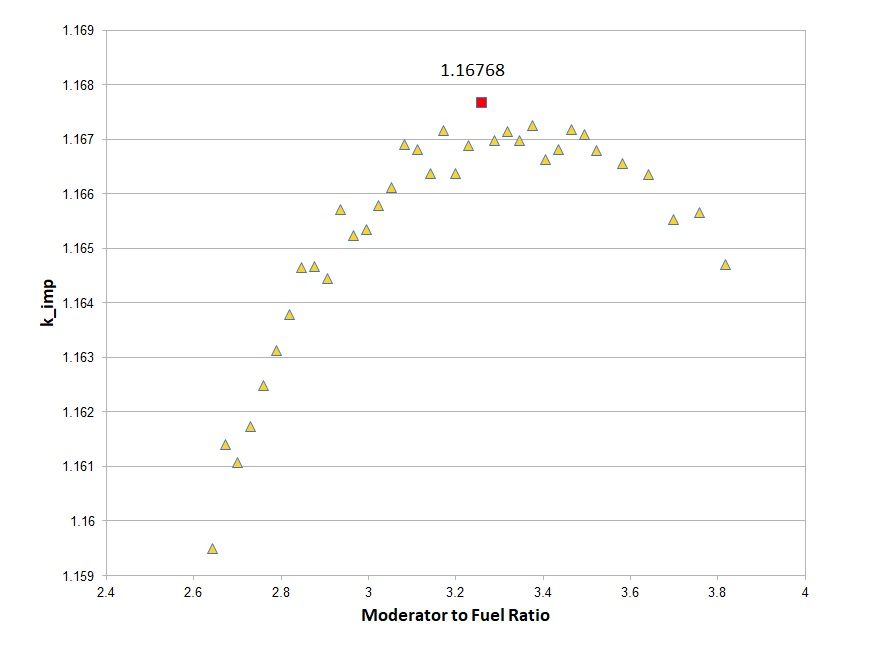
\includegraphics[scale=0.6]{plot}
\caption{K\_IMP from Serpent output plotted against Moderator to Fuel ratio, for moderator density ranging from 0.9 to 1.3 g/mL.}
\end{figure}

\pagebreak

\section{Serpent Input File corresponding to optimum moderator to fuel ratio}

\begin{lstlisting} [ basicstyle=\tiny]
% --- Pin-cell burnup calculation ----------------------------
set title "Pin-cell burnup calculation"

% --- Pin definition:
pin 1
fuel 0.469550
void 0.479100
clad 0.546400
water

% --- Geometry:
surf 1 sqc 0.0 0.0 0.721350
cell 1 0 fill 1 -1
cell 2 0 outside 1

% --- Fuel (composition in atom fraction):
mat fuel  -10.21
92235.09c   0.005000
92238.09c   0.328333
 8016.09c   0.666667

% --- Zircalloy cladding (composition in mass fraction)
mat clad  -6.560
40000.06c -0.9823
50000.06c -0.0145
26000.06c -0.0021
24000.06c -0.0010
72000.06c -0.0001

% --- Water (composition in atom fraction):
mat water -1.1100 moder lwtr 1001
1001.06c   0.666667
8016.06c   0.333333

% --- Thermal scattering data for light water:
therm lwtr lwe7.10t

% --- Periodic boundary condition:
set bc 3

% --- Group constant generation:
% universe = 0 (homogenization over all space)
% 2-group structure (group boundary at 0.625 eV)
set gcu 0
set nfg 2 0.625E-6

% --- Geometry and mesh plots:
plot 3 1000 1000
mesh 3 1000 1000

% --- Cross section library file path:
set acelib "/home/serpent/xs/endfb7/sss_endfb7.xsdata"
set declib "/home/serpent/xs/endfb7/sss_endfb7.dec"
set nfylib "/home/serpent/xs/endfb7/sss_endfb7.nfy"

% --- Reduce energy grid size:
set egrid 5E-5 1E-10 15.0

% --- Depletion steps:
% Cycle 1
set powdens 25.00E-3

% --- Neutron population and criticality cycles:
set pop 10000  200  20

\end{lstlisting}

\end{document}
